\documentclass[a4paper,11pt]{article}
\usepackage[margin=0.9in]{geometry}
\usepackage{calc}
\usepackage{wrapfig}
\usepackage{scrextend}
\usepackage{xspace}
\usepackage{float}
\usepackage{array}
\usepackage{booktabs}
\usepackage{adjustbox}
\usepackage{bigdelim}
\usepackage{rotating}

\newenvironment{aside}
    {\begin{mdframed}[
        leftline=false,rightline=false,leftmargin=2em,rightmargin=2em,
        innerleftmargin=0pt,innerrightmargin=0pt,linewidth=0.75pt,
        skipabove=7pt,skipbelow=7pt]\small}
    {\end{mdframed}}


% Set up equations
\usepackage{amsmath}

% half-transparent percentage command
\newcommand{\p}{\,\textcolor{gray}{\%}\xspace}

% Configure lists
\usepackage{enumitem}
\setlist[itemize]{topsep=0pt}
\setlist[enumerate]{topsep=0pt}

% Configure figures
\renewcommand{\figurename}{Figure}
\renewcommand{\floatpagefraction}{.99}

% Custom icons
\usepackage{fontspec}
\newfontfamily\iconsfont{icons.ttf}
\newcommand{\iconDocker}{\raisebox{-0.5ex}{{\iconsfont a}}\xspace}
\newcommand{\iconGoogleDrive}{\raisebox{-0.4ex}{{\iconsfont b}}\xspace}

% Add github/dockerhub commands
\usepackage{fontawesome}
\newcommand{\github}[2]{\,\href{https://github.com/#1/#2}{\faGithub~#1/\linebreak[0]#2}\xspace}
\newcommand{\dockerhub}[2]{\,\href{https://hub.docker.com/repository/docker/#1/#2}{\iconDocker~#1/\linebreak[0]#2}\xspace}

% Configure diagrams
\usepackage{tikz}
\tikzset{every picture/.style={line width=0.75pt}} 

% Colors
\usepackage{xcolor}
\definecolor{seablue}{HTML}{2A5DB0}
\definecolor{cardinalred}{HTML}{C41E3A}
\definecolor{avocadogreen}{HTML}{446604}
\definecolor{moby}{rgb}{0.2, 0.4, 0.6}
\definecolor{radvisor}{rgb}{0.9, 0.2, 0.2}

% Configure bibliography
\usepackage[style=ieee]{biblatex}
\usepackage[colorlinks = true,
            linkcolor = black,
            urlcolor  = seablue,
            citecolor = black,
            anchorcolor = seablue]{hyperref}
\addbibresource{citations.bib}
\setcounter{biburllcpenalty}{7000}
\setcounter{biburlucpenalty}{8000}

% Remove empty parens on IEEE @online citations without years
\usepackage{xpatch}
\xpatchbibdriver{online}
  {\printtext[parens]{\usebibmacro{date}}}
  {\iffieldundef{year}
    {}
    {\printtext[parens]{\usebibmacro{date}}}}
  {}
  {\typeout{There was an error patching biblatex-ieee (specifically, ieee.bbx's @online driver)}}
  
% Adjust various spaces
\setlength{\headsep}{0.75em}
\setlength{\parindent}{0pt}
\setlength{\parskip}{1em}
\usepackage[skip=2pt]{caption}
\setlength{\belowcaptionskip}{-16pt}

% Change title spacing to reduce spacing after headings
\usepackage{titlesec}
\titlespacing{\section}{0pt}{-0.6em + \parskip}{-\parskip + 0.65em}
\titlespacing{\subsection}{0pt}{-0.9em + \parskip}{-\parskip + 0.55em}
\titlespacing{\subsubsection}{0pt}{-1em + \parskip}{-\parskip + 0.45em}

\title{
    \vspace{-1.35em}
    \textbf{\huge{CS-4365 Final Report}}\\[1pt]
    System Resource Utilization Monitoring for Docker Containers
    \vspace{-0.5em}
}
\author{Joseph Azevedo and Bhanu Garg}
\date{\vspace{-0.7em}\vspace{-\parskip}April 2020}

% Set up tables
\usepackage{ragged2e}
\newcolumntype{L}[1]{>{\raggedright\let\newline\\\arraybackslash\hspace{0pt}}m{#1}}
\newcolumntype{C}[1]{>{\centering\let\newline\\\arraybackslash\hspace{0pt}}m{#1}}
\newcolumntype{R}[1]{>{\raggedleft\let\newline\\\arraybackslash\hspace{0pt}}m{#1}}

% Configure code snippets
\usepackage{minted}
\usepackage{xargs}
\usemintedstyle{friendly}
\setminted{fontsize=\small, linenos, tabsize=2, breaklines, numbersep=18pt}
\usepackage[framemethod=TikZ]{mdframed}
\definecolor{codebg}{HTML}{fafafa}
\definecolor{codelinenums}{HTML}{575961}
\newcommandx{\code}[3][1=text, 2=\small]{
    \begin{mdframed}[
        backgroundcolor = codebg,
        linewidth = 1.5pt,
        linecolor = black!9,
        roundcorner = 6pt
    ]
        \renewcommand{\theFancyVerbLine}{\textcolor{codelinenums!60}{\footnotesize{\arabic{FancyVerbLine}}}}
        \inputminted[fontsize=#2]{#1}{#3}
    \end{mdframed}
}

% Configure breakable teletype filepaths
\newcommand{\filepath}[1]{\texttt{#1}\xspace}

% Common terms
\newcommand{\granularitybf}{\textbf{high granularity}\xspace}
\newcommand{\granularity}{\textit{high granularity}\xspace}
\newcommand{\overheadbf}{\textbf{low overhead}\xspace}
\newcommand{\overhead}{\textit{low overhead}\xspace}
\newcommand{\dockerstats}{\texttt{docker stats}\xspace}

\begin{document}

\maketitle

\vspace{-\parskip}
\vspace{-2em}
\section{Introduction}

In recent years, the use of containerization in enterprise systems has skyrocketed as software teams adopt the technology
to increase developer agility and simplify deployment.
Tools like Docker allow developers to build and deploy their applications in reproducible environments \cite{Docker-Overview},
proving to be extremely useful as many companies move their applications to the cloud.
Overall industry usage of containerization technologies has jumped from just over half at 55\% in 2017 to 87\% in 2019 \cite{Portworx},
and this trend is unlikely to slow down. With this, many solutions have emerged for monitoring containers,
such as Sysdig, which describes itself as a ``Linux system exploration and troubleshooting tool
with first class support for containers'' \cite{SysDig}, 
promising to allow users to closely monitor container system resource utilization. Another is Google's own cAdvisor,
which advertises itself as a tool for analyzing ``resource usage and performance characteristics of running containers'' \cite{Cadvisor}.
While these tools work well for their intended purposes, which range from deep system introspection to cloud-native deployment monitoring,
they fall flat when there is a need to analyze resource utilization with both \granularity and \overhead---%
something that most tools only provide one of.

An example of a scenario where we need this is when studying the phenomenon of millibottlenecks in containerized systems.
First introduced by Pu et al. in The Millibottleneck Theory of Performance Bugs, and Its Experimental Verification,
the millibottleneck theory of performance bugs explains that the long tail problem and its underlying cause, millibottlenecks,
are caused by very short resource bottlenecks that then propagate through an application system
and become amplified due to dependencies and their effect on downstream components \cite{Millibottleneck}.
These resource bottlenecks can be caused by a variety of different hardware and software events,
such as garbage collection in managed languages or CPU clock speed governors being slow to ramp up during intense bursts of system load.
No matter the cause, though, they tend to become aggrandized as the system continues,
producing abnormally long response times before the system recovers shortly thereafter
and returns to exhibiting standard response times.
This results in a so-called ``long tail problem,''
which appears to web service consumers as unusually long response times for a small proportion of requests \cite{Tail-At-Scale}.
Requiring high performance in a scalable system like Google’s parallel search system decreases tolerance levels,
so these degradations are unacceptable to the companies running these services.
In fact, Google reported a loss in up to 20\% of revenue from request latencies of 500 milliseconds \cite{Google}.
Another example of the effect of latency long tail is seen through Amazon sales—--
they found that every 100 milliseconds of delay in page loading correlates to a 1\% loss of sales \cite{Millibottleneck}. 

Because these millibottlenecks occur over relatively short intervals (on the scale of tens or hundreds of milliseconds),
most monitoring tools are incapable of capturing their effects
while simultaneously maintaining low enough overhead as to not impact the measured performance.
The situation gets even more complicated when attempting to analyze millibottlenecks in containerized environments,
where traditional monitoring methods don't work as expected inside containers.
Instead, in order to effectively monitor container resource utilization,
you need a custom tool that is able to run on a system and collect information on all running containers.
This comprises the main focus of our project,
where we investigate various tools for instrumenting Docker containers
and ultimately develop our own custom solution in Rust (\textit{see Implementation}).

\vspace{-0.1em}
\subsection{Docker}

As a technology, containerization provides many benefits to enterprise systems,
allowing developers to package applications along with their process-level configuration and dependencies as a single unit,
called an image.
Then, by using tools such as the Docker runtime, these images can be instantiated as configured processes, called containers,
that exist on a host machine as a virtualized environment/runtime.
Compared to standard virtualization, containerization is significantly more lightweight,
as the Docker runtime directly utilizes the kernel of the host operating system
while maintaining a high level of security and isolation \cite{Docker-Overview}.
Overall, Docker makes it very easy to deploy applications as containers on a variety of different infrastructures,
from managed clouds to on-premise clusters (Figure \ref{fig:docker_stack}).

% Docker stack diagram
\setlength\intextsep{-0.3em}
\begin{wrapfigure}{r}{0.46\textwidth}
    \scalebox{}{}
    \begin{addmargin}[0.5em]{0em}
        \resizebox{\linewidth}{!}{\input{diagrams/Docker_stack.tex}}
        \vspace{-0.25em}
        \caption{Docker engine architecture, showing multiple applications residing on a single host OS}
        \label{fig:docker_stack}
    \end{addmargin}
    \vspace{1.2em}
\end{wrapfigure}

Nonetheless, containerization presents additional challenges when it comes to monitoring resource utilization for applications.
Because it uses virtualization at the operating system level (as opposed to the hardware level),
it becomes easy to run multiple containers on one host operating system,
better maximizing resource utilization.

This causes many of the resource monitoring techniques used in bare metal or virtualized environments
(especially those used to detect and analyze millibottlenecks)
to not be effective anymore, as they often operate on the operating system level.
For example, Collectl is one of the tools of choice for monitoring CPU, memory, and disk I/O utilization
for the Elba project \cite{ElbaRodrigo} (a research team investigating the emergence and propagation of millibottlenecks),
as it is able to record data at a high resolution while maintaining a \overhead.
Collectl records these statistics for system-wide utilization \cite{Collectl},
which, while useful when there is only one application running on a single machine or VM,
is much less useful when there are multiple containerized application instances running on one host operating system.
The search to find a specialized tool that is able to monitor resource utilization
at the level of individual containers became one of the main focuses of our project.

\setlength\intextsep{1.2em}
\vspace{-0.28em}
\section{Project evolution}

The original intent of our project was to adapt the WISE microblog benchmark \cite{microblog} to run under Docker
and Kubernetes, an orchestration platform for managing complex Docker-based deployments \cite{Kubernetes}.
Through this, we hoped to monitor latency delays
and potentially discover differences in the ways millibottlenecks emerge in scalable systems. 

To accomplish this, we needed a tool that was capable of monitoring the system resource utilization
of running Docker containers, and it had to operate with:

\vspace{-0.18em}
\begin{enumerate}
    \item \granularitybf, which relates to the consistency and precision of collection interval,
    even under medium and high loads.
    According to the Nyquist–Shannon Sampling Theorem,
    we can reliably monitor events of at least 100ms in length with a 50ms monitoring interval \cite{SamplingTheorem},
    which corresponds to the general timescale of millibottlenecks \cite{Millibottleneck}.
    
    \item \overheadbf, which relates to the act of collection having a relatively low impact on application performance.
    This is important to reduce the amount of bias caused by collection in the final results.
\end{enumerate}
\vspace{-0.25em}

These comprised the primary criteria we were using when evaluating potential solutions,
and we set out to find a tool that provided both while working on the level of individual containers.

\subsection{\dockerstats}

The first tool we evaluated for monitoring Kubernetes pods was the built-in Docker resource monitor.
While testing the internal Docker CLI tool, \dockerstats, we noticed some pros and cons.
\dockerstats is native to Docker, which would require no excessive modification from our end to use in experiments.
However, the tool is set to poll the Docker engine every one second for up-to-date usage stats in JSON format,
and this interval can not be decreased.
Due to the extensively long polling interval, it is impossible to achieve the high granularity required for the project. 

\subsection{cAdvisor}

The next tool we examined was cAdvisor,
which is a command line tool developed by Google and geared toward system administrators.   
It operates as a background daemon, similar to the Docker engine, where it collects statistics about running containers,
including ``resource isolation parameters, historical resource usage,
histograms of complete historical resource usage and network statistics'' \cite{Cadvisor}.
However, it was difficult to obtain our desired goals when using it.
cAdvisor provides both a web-based GUI tool for viewing statistics and a high-granularity output log.
The web-based interface provides useful information,
but collects at relatively high intervals around 1 second and is difficult to extract information from. 
Its output log, on the other hand, provided high granularity, but also monitored much more than just running containers,
meaning its overhead would be significantly more than a tool that just instruments containers (Figure \ref{fig:cadvisor_out}).

% Example snippet from https://github.com/elba-docker/instrumentation/blob/master/cadvisor/output.txt
\begin{figure}[H]
    % minted doesn't support generic logs, so just use a language that looks okay
    
    \code[python]{snippets/cadvisor.out}
    \caption{
        Code snippet showing data collected using cAdvisor.
        The output is excessive, showing statistics collected for cgroups completely unrelated to Docker.
    }
    \label{fig:cadvisor_out}
\end{figure}

\subsection{Sysdig}

Sysdig is another tool built toward letting system administrators monitor fine-tuned performance of a single machine,
providing high granularity but coming at the cost of high overhead.
Sysdig, unlike the internal Docker CLI tool, allowed for adjustable collection intervals,
but had a lower limit at 100ms \cite{SysDigLimit}.
Since our target collection frequency was 50ms,
we had to make a short patch and recompile the binary to remove the restriction
(at \github{elba-docker}{sysdig}).
The base CLI tool, \texttt{sysdig}, outputs all syscalls,
which is significantly more granularity than we need and is not useful for our monitoring purposes.
In addition, intercepting all syscalls introduces significant overhead that we needed to avoid in our monitoring tool (Figure \ref{fig:sysdig_out}).

\begin{figure}
    % minted doesn't support generic logs, so just use a language that looks okay
    \code[python]{snippets/sysdig.out}
    \caption{
        Code snippet showing data collected using \texttt{sysdig container.image=ubuntu}.
        The output shows all syscalls related to a single container, which, while informative, is undesired for our use case.
    }
    \label{fig:sysdig_out}
    \vspace{1em}
\end{figure}

Sysdig also offers a curses-based CLI tool (Figure \ref{fig:csysdig}), \texttt{csysdig},
but it is unclear how to translate the given outputs to a log file,
which is needed to later analyze how millibottlenecks emerge in and affect an online system.
Moreover, despite changing the collection interval to 50 milliseconds with the command-line flag \texttt{-d 50},
the resultant display only updated the CPU utilization each second,
suggesting that there is a hidden limit to how much granularity the tool provides.

\begin{figure}[H]
    \centering
    \includegraphics[width=\textwidth]{images/csysdig.png}
    \vspace{-0.3em}
    \caption{
        Example output of the \texttt{csysdig} monitoring tool in container mode,
        showing its curses-based interface. The command used is \texttt{csysdig -vcontainers}.
    }
    \label{fig:csysdig}
\end{figure}

Ultimately, we were not able to find an existing tool
that provided the necessary combination of \granularity and \overhead,
so we looked into modifying an existing tool.

\subsection{Moby}

Moby is an open-source framework that is the core of the Docker engine and is built in Golang. 
It runs as a daemon on the host system where the Docker CLI tool communicates with it through Unix sockets. 
Because it already contained a backend implementation for \dockerstats,
which almost satisfied our requirements but lacked granularity,
we looked toward modifying Moby to increase its collection granularity.
After forking Moby on GitHub, we added a configuration option for the \dockerstats collection interval
to control the collection granularity.
We then proceeded to add functionality that outputs utilization logs for all running containers
and changed it to output CSV instead of JSON.
Although we were able to make adjustments to Moby,
there were still drawbacks that prevented us from using it.
Moby presented difficulties in measuring overhead due to it being a part of the core Docker runtime,
which meant there was no control for users to start and stop it because it is always running.
Our patch also adds complexity to already-complex software and can not be easily generalized to include Kubernetes metadata,
one of the goals of our project at that time.
Another concern with Moby was the difficulty involved with maintaining a fork
that could face problems with security patches in the future.
Finally, Moby faces inherent problems due to being built in Golang,
which, while much faster than other interpreted languages like Python,
still uses a built-in garbage collector,
leading to unpredictable and inconsistent resource utilization in the instrument itself.

Due to the limitations faced with Moby, we decided to build our own tool called rAdvisor (a play on Google's cAdvisor),
a Rust-based tool designed to achieve \granularity and \overhead.
From this, we were able to compare its performance with Moby to evaluate whether it achieves its goal
and has the potential to be a useful tool in detecting and analyzing millibottlenecks in containerized environments.
 
\section{Implementation}

\subsection{Moby}

Moby, as discussed earlier, is the Docker core engine (built in Golang) which we forked to \github{elba-docker}{moby}
and modified to add custom collection configuration and behavior.
The first modification was to use the existing configuration framework
that loads the daemon configuration from a JSON file at \filepath{/etc/docker/daemon.json} (Figure \ref{fig:moby_config}).
Afterward, we replaced the hard-coded collection interval for \dockerstats (which was originally 1 second)
with the value loaded from the config (in milliseconds).
By doing this, we were able to adjust the collection granularity at runtime by changing a single line in the config file,
instead of having to recompile the engine from source.

\begin{figure}[H]
    \code[json]{snippets/config.json}
    \caption{
        Sample Docker daemon configuration used in our experiments
        (\href{https://github.com/elba-docker/experiment/blob/a39daa1bb4b742c974a43f3d5e44f6036d1d16ad/experiments/direct_collectl/scripts/run.sh\#L117-L125}{source}),
        showing the added configuration option to change the \dockerstats collection interval (line 8)
    }
    \label{fig:moby_config}
\end{figure}

% i don't like even still as the beginning to the paragraph
Even still, there were more improvements to be made.
For one, \dockerstats uses a long-lived HTTP connection to stream stats that is unnecessary in our case
and needs to be started/stopped either manually or by some other tool
each time the set of running containers changes.
To alleviate this, we introduced an automatic collection extension
that leverages one of Golang's first-class concurrency control units, Goroutines \cite{GolangGoroutines}.
These functions, which act as light-weight threads,
allow us to dispatch a new collector every time a new container starts that runs in the background,
getting stopped when the associated container finally stops.
Then, we re-use the streaming functionality implemented in \dockerstats
and redirect the output to write to a buffered writer in front of a file
at \filepath{/var/logs/docker/stats/\{id\}.log}.
The buffered writer is necessary to reduce the frequency of writes at runtime,
which lowers the overhead of collection
(a similar technique is employed in the Elba project's WISETrace,
which intercepts and logs network syscalls as a kernel module \cite{milliScope}).

Another performance-increasing modification we made is switching
from the JSON stats serializer used for the \dockerstats API backend
to a more basic serializer that uses CSV.
This resulted in a speed increase when marshalling the statistics struct
by a factor of 2.335 (Table \ref{tab:stats_benchmark}).

\begin{table}
    \vspace{1em}
    \caption{
        Benchmark (\href{https://github.com/elba-docker/instrumentation/blob/master/moby/benchmarks/stats_test.go}{source})
        results for serializing a single \texttt{StatsJSON} struct
        using both JSON (original) and CSV (modified) targets.
        The test was ran on Ubuntu 20.04 LTS with an Intel Pentium G3258 and 8GB RAM.
    }
    \vspace{1em}
    \centering
    \begin{tabular}{L{3.2cm} R{2.3cm} R{3.3cm}}
        \toprule
        \textbf{Test} & \textbf{Number of operations} & \textbf{Execution speed (ops/sec)} \\
        \midrule
        JSON Serialization & 883,716  & 27,475 \\
        \midrule
        CSV Serialization  & 2,034,567 & 11,769 \\
        \bottomrule
    \end{tabular}
    \label{tab:stats_benchmark}
\end{table}

\newcommand{\newcolor}{avocadogreen}
These functional changes can be summarized by Figure \ref{fig:moby_sequence},
a sequence diagram showing the lifecycle of container statistics collection.

\begin{figure}
    \centering
    \vspace{1.5em}
    \begin{tikzpicture}[>=stealth]

\newcommand{\id}{\texttt{d58fe}\xspace}

% Locations
\def\ClientToDaemon{++(5,0)}
\def\DaemonToClient{++(-5,0)}
\def\DaemonToGoroutine{++(5,0)}
\def\GoroutineToDaemon{++(-5,0)}
\def\Lifeline{++(0,-7.75)}

% Lifelines
\path (0,0)              node[draw, fill=seablue!10]     (Client)    {API Client}
      \ClientToDaemon    node[draw, fill=seablue!10]     (Daemon)    {Daemon}
      \DaemonToGoroutine node[draw, fill=\newcolor!10,draw=\newcolor,text=\newcolor!30!black] (Goroutine) {Collection goroutine for \id};
\draw [dotted] (Client) -- \Lifeline (Daemon) -- \Lifeline (Goroutine) -- \Lifeline;

% Flows
\path (Client)
      ++(0,-0.75) node (BeginClient)      {}
      ++(0,-0.25) node (BeginClientStart) {}
      ++(0,-1.75) node (EndClientStart)   {}
      ++(0,-0.25) node (EndClientInit)    {}
      ++(0,-2.25) node (BeginClientExit)  {}
      ++(0,-0.25) node (BeginClientStop)  {}
      ++(0,-1.75) node (EndClientStop)    {}
      ++(0,-0.25) node (EndClient)        {};
\path (Daemon)
      ++(0,-1)    node (BeginStart)          {}
      ++(0,-0.25) node (BeginSelfStart)      {}
      ++(0,-0.5)  node (EndSelfStart)        {}
      ++(0,-0.75) node (BeginGoroutineStart) {}
      ++(0,-0.25) node (EndStart)            {}
      ++(0,-2.75) node (BeginStop)           {}
      ++(0,-0.25) node (BeginSelfStop)       {}
      ++(0,-0.5)  node (EndSelfStop)         {}
      ++(0,-0.75) node (BeginGoroutineStop)  {}
      ++(0,-0.25) node (EndStop)             {};
\path (Goroutine)
      ++(0,-2.5)   node (BeginGoroutine)   {}
      ++(0,-0.25)  node (BeginSelfOpen)    {}
      ++(0,-0.5)   node (EndSelfOpen)      {}
      ++(0,-0.5)   node (BeginLoop)        {}
      ++(0,-0.95)  node (BeginSelfSleep)   {}
      ++(0,-0.5)   node (EndSelfSleep)     {}
      ++(0,-0.5)   node (BeginSelfCollect) {}
      ++(0,-0.5)   node (EndSelfCollect)   {}
      ++(0,-0.825) node (EndGoroutine)     {};

% Blocks
\filldraw[fill=seablue!30]                  (BeginClient.west)     rectangle (EndClientInit.east);
\filldraw[fill=seablue!30]                  (BeginStart.west)      rectangle (EndStart.east);
\filldraw[fill=\newcolor!30,draw=\newcolor] (BeginGoroutine.west)  rectangle (EndGoroutine.east);
\filldraw[fill=seablue!30]                  (BeginClientExit.west) rectangle (EndClient.east);
\filldraw[fill=seablue!30]                  (BeginStop.west)       rectangle (EndStop.east);

% Calls
\draw[->]         (BeginClientStart.east)    -- node[above,text depth=.5pt]    {\texttt{docker start \id}} (BeginStart.west);
\draw[->][dashed] (EndStart)                 -- node[above,text depth=.5pt]    {Successful} (EndClientStart);
\draw[->]         (BeginSelfStart)           -- ++(1, 0) node (SelfStartTop)   {} -- node[right=1pt,text depth=1pt] {start container} ++(0, -0.5) node (SelfStartBottom) {} -- (EndSelfStart);
\draw[->][draw=\newcolor]         (BeginGoroutineStart.east) -- node[above,text depth=.5pt,text=\newcolor]    {\texttt{go StartStatsLogs()}} (BeginGoroutine.west);
\draw[->]         (BeginClientStop.east)     -- node[above,text depth=.5pt]    {\texttt{docker stop \id}} (BeginStop.west);
\draw[->][dashed] (EndStop)                  -- node[above,text depth=.5pt]    {Successful} (EndClientStop);
\draw[->]         (BeginSelfStop)            -- ++(1, 0) node (SelfStopTop)    {} -- node[right=1pt,text depth=1pt] {stop container} ++(0, -0.5) node (SelfStopBottom) {} -- (EndSelfStop);
\draw[->][draw=\newcolor]         (BeginGoroutineStop.east)  -- node[above,text depth=.5pt,text=\newcolor]    {\texttt{StopStatsLogs()}} (EndGoroutine.west);
\draw[->][draw=\newcolor]         (BeginSelfOpen)            -- ++(1, 0) node (SelfOpenTop)    {} -- node[text=\newcolor,right=1pt,text depth=1pt] {open log file} ++(0, -0.5) node (SelfOpenBottom) {} -- (EndSelfOpen);
\draw[->][draw=\newcolor]         (BeginSelfSleep)         -- ++(1, 0) node (SelfSleepTop) {} -- node[text=\newcolor,right=1pt,text depth=1pt] {sleep for interval} ++(0, -0.5) node (SelfSleepBottom) {} -- (EndSelfSleep);
\draw[->][draw=\newcolor]         (BeginSelfCollect)         -- ++(1, 0) node (SelfCollectTop) {} -- node[text=\newcolor,right=1pt,text depth=1pt] {collect to CSV} ++(0, -0.5) node (SelfCollectBottom) {} -- (EndSelfCollect);

% Loop
\draw[draw=\newcolor] (BeginLoop.west) ++(-0.375,0) rectangle ++(4.875,-2.75);
\draw (BeginLoop.west) ++(-0.375,0) node[anchor=north west,fill=white,draw=\newcolor,fill opacity=0.8,text=\newcolor!30!black,text opacity=1] {loop};

\end{tikzpicture}

    \vspace{0.625em}
    \caption{
        Simplified sequence diagram of the modifications made to Moby
        to allow for fine-grained container monitoring.
        Additions we made to the Moby engine are highlighted in \textcolor{\newcolor}{green}.
    }
    \label{fig:moby_sequence}
    \vspace{1em}
\end{figure}

\pagebreak
\subsubsection{Packaging}

To deploy our patched version of Moby, we used the existing build tools in \github{docker}{docker-ce}
(the repository used to build the standard Docker packages)
to build our own \texttt{.deb} packages for Docker and Docker CLI.
We then used the generated packages
(\textit{see Appendix \ref{app:artifacts}})
to deploy our patched version in our experiments.

\subsection{rAdvisor}

With the limitations we observed in our patched version of Moby,
we created rAdvisor to attempt to overcome them.
Our goal with rAdivsor was to create a tool that collects resource utilization statistics on all running containers
and outputs it in a useful format, similar to Collectl.
During development, we sought to specifically address the shortcomings of Moby
in the way we designed rAdvisor.
For one, it is an extremely focused tool---%
its sole purpose is to instrument running containers---%
so it is easier to debug, maintain, and limit the performance impact of.
This also means it is much easier to measure its overhead,
which we attempted to do via experimental observation (\textit{see Evaluation}).
Its source code can be found in its corresponding repository on GitHub:
\github{elba-docker}{radvisor}.

The tool was built using the Rust language, which is a statically-typed, C-like language
intended for memory-safe programming.
Our reasoning behind picking Rust was because it is a low level language with similar performance to C,
ultimately allowing for lower overhead \cite{TheRustBook}.
Compared to Golang, Rust has no garbage collector,
allowing for greater consistency in sampling
due to the lack of short resource usage peaks
that themselves have been shown to cause short-lived resource bottlenecks \cite{Millibottleneck}.
It also provides many benefits over C, such as its purpose-built type system and compiler
that are able to effectively eliminate runtime memory errors.

\subsubsection{Structure}

rAdvisor runs in the background and collects statistics for active containers at a configurable collection interval.
The tool leverages the advanced concurrency capabilities of Rust,
utilizing two main threads (Figure \ref{fig:radvisor_sequence}) that accomplish its purpose
by communicating across a single, shared channel:

\vspace{-0.2em}
\begin{enumerate}
    \item The \textbf{polling thread} polls the Docker daemon API through a Unix socket at a configurable interval
    to get a list of active and running containers.
    The thread then filters and processes the list,
    and sends events (add or remove) to the collection thread utilizing the cross-thread channel.
    
    \item The \textbf{collection thread} runs at a configurable interval
    and reads a set of files in the cgroupfs pseudo-filesystem using Linux cgroups.
    The thread then writes their contents to a buffered CSV writer
    that eventually writes to a file in \filepath{/var/log/radvisor/stats} each time the buffer is flushed.
    This is done for every container in the list of active containers,
    which is determined by the incoming events sent from the polling thread.
    The collection interval is separate from the polling interval,
    and is generally much shorter (the default is 50 milliseconds versus 1 second for the polling thread).
    This is because the list of active containers changes fairly infrequently,
    whereas the goal of the tool is to collect container resource utilization
    with \granularity.
\end{enumerate}
\vspace{0.2em}

\newcommand{\polling}{seablue}
\newcommand{\collection}{cardinalred}
\begin{figure}[h]
    \centering
    \begin{adjustbox}{max width=\textwidth}
    \begin{tikzpicture}[>=stealth]
    
    \newcommand{\shared}{\collection!50!\polling}
    
    % Locations
    \def\Lifeline{++(0,-6.5)}
    
    % Lifelines
    \path (0,0)     node[draw, fill=\polling!10]    (Polling)    {Polling Thread}
          ++(5,0)   node[draw, fill=\polling!10]    (Docker)     {Docker Daemon}
          ++(2.5,0) node[draw, fill=\shared!10]     (Channel)    {Channel}
          ++(3.5,0) node[draw, fill=\collection!10] (Collection) {Collection Thread}
          ++(4,0)   node[draw, fill=\collection!10] (Cgroupfs)   {cgroupfs};
    \draw [dotted] (Polling) -- \Lifeline (Docker) -- \Lifeline (Channel) -- \Lifeline (Collection) -- \Lifeline (Cgroupfs) -- \Lifeline;
    
    % Flows
    \path (Polling)
          ++(0,-0.75) node (PollingLoop)       {}
          ++(0,-0.5)  node (BeginPolling)      {}
          ++(0,-0.75) node (BeginPollingPoll)  {}
          ++(0,-0.75) node (ReturnPollingPoll) {}
          ++(0,-1)    node (BeginPollingPost)  {}
          ++(0,-0.5)  node (ReturnPollingPost) {}
          ++(0,-0.5)  node (BeginPollingSleep) {}
          ++(0,-0.5)  node (EndPollingSleep)   {}
          ++(0,-0.25) node (EndPolling)        {};
    \path (Docker)
          ++(0,-1.75) node (BeginDocker)      {}
          ++(0,-0.25) node (BeginDockerPoll)  {}
          ++(0,-0.75) node (ReturnDockerPoll) {}
          ++(0,-0.25) node (EndDocker)        {};
    \path (Channel)
          ++(0,-1.5)  node (BeginChannelPoll)  {}
          ++(0,-0.75) node (ReturnChannelPoll) {}
          ++(0,-1.5)  node (BeginChannelPost)  {}
          ++(0,-0.5)  node (ReturnChannelPost) {};
    \path (Collection)
          ++(0,-0.75) node (CollectionLoop)        {}
          ++(0,-0.5)  node (BeginCollection)       {}
          ++(0,-0.25) node (BeginCollectionPoll)   {}
          ++(0,-0.75) node (ReturnCollectionPoll)  {}
          ++(0,-0.5)  node (BeginCollectionUpdate) {}
          ++(0,-0.5)  node (EndCollectionUpdate)   {}
          ++(0,-0.75) node (BeginCollectionRead)   {}
          ++(0,-0.75) node (ReturnCollectionRead)  {}
          ++(0,-0.5)  node (BeginCollectionSleep)  {}
          ++(0,-0.5)  node (EndCollectionSleep)    {}
          ++(0,-0.25) node (EndCollection)         {};
    \path (Cgroupfs)
          ++(0,-4)    node (BeginCgroupfsRead)  {}
          ++(0,-0.75) node (ReturnCgroupfsRead) {};
    
    % Blocks
    \filldraw[fill=\polling!30]    (BeginPolling.west)      rectangle (EndPolling.east);
    \filldraw[fill=\polling!30]    (BeginDocker.west)       rectangle (EndDocker.east);
    \filldraw[fill=\shared!30]     (BeginChannelPoll.west)  rectangle (ReturnChannelPoll.east);
    \filldraw[fill=\shared!30]     (BeginChannelPost.west)  rectangle (ReturnChannelPost.east);
    \filldraw[fill=\collection!30] (BeginCollection.west)   rectangle (EndCollection.east);
    \filldraw[fill=\collection!30] (BeginCgroupfsRead.west) rectangle (ReturnCgroupfsRead.east);
    
    % Calls
    \draw[->]         (BeginPollingPoll)      -- node[above,text depth=.5pt] {get running containers} (BeginDockerPoll);
    \draw[->][dashed] (ReturnDockerPoll)      -- node[above,text depth=.5pt] {container list}         (ReturnPollingPoll);
    \draw[->]         (BeginPollingPost)      -- node[above,text depth=.5pt] {post add/remove events} (BeginChannelPost);
    \draw[->][dashed] (ReturnChannelPost)     -- node[above,text depth=.5pt] {}                       (ReturnPollingPost);
    \draw[->]         (BeginCollectionPoll)   -- node[above,text depth=.5pt] {get new events}         (BeginChannelPoll);
    \draw[->][dashed] (ReturnChannelPoll)     -- node[above,text depth=.5pt] {event list}             (ReturnCollectionPoll);
    \draw[->]         (BeginCollectionRead)   -- node[above,text depth=.5pt] {read cgroup stats}      (BeginCgroupfsRead);
    \draw[->][dashed] (ReturnCgroupfsRead)    -- node[above,text depth=.5pt] {stats}                  (ReturnCollectionRead);
    \draw[->]         (BeginPollingSleep)     -- ++(1, 0) node (PollingSleepTop)     {} -- node[right=1pt,text depth=1pt] {sleep (polling interval)}    ++(0, -0.5) node (PollingSleepBottom)     {} -- (EndPollingSleep);
    \draw[->]         (BeginCollectionUpdate) -- ++(1, 0) node (CollectionUpdateTop) {} -- node[right=1pt,text depth=1pt] {update active containers}    ++(0, -0.5) node (CollectionUpdateBottom) {} -- (EndCollectionUpdate);
    \draw[->]         (BeginCollectionSleep)  -- ++(1, 0) node (CollectionSleepTop)  {} -- node[right=1pt,text depth=1pt] {sleep (collection interval)} ++(0, -0.5) node (CollectionSleepBottom)  {} -- (EndCollectionSleep);
    
    % Loop
    \draw (PollingLoop.west)    ++(-0.625,0) rectangle ++(6.75,-5);
    \draw (PollingLoop.west)    ++(-0.625,0) node[anchor=north west,fill=white,fill opacity=0.6,text opacity=1,draw=black] {loop};
    \draw (CollectionLoop.west) ++(-4.45,0)  rectangle ++(10.4,-5.55);
    \draw (CollectionLoop.west) ++(-4.45,0)  node[anchor=north west,fill=white,fill opacity=0.6,text opacity=1,draw=black] {loop};
    
    \end{tikzpicture}
\end{adjustbox}

    \vspace{-0.5em}
    \caption{
        Simplified sequence diagram of the concurrent architecture of rAdvisor.
        Operations related to the \textit{polling thread} are \textcolor{\polling}{blue};
        operations related to the \textit{collection thread} are \textcolor{\collection}{red}.
    }
    \label{fig:radvisor_sequence}
    \vspace{1em}
\end{figure}

\subsubsection{Implementation Details}

As mentioned before, the implementation of the collection functionality heavily relies on Linux cgroups.
Added to the Linux kernel version 2.6.24 in 2008 \cite{CgroupsVer},
cgroups are one of the core technologies that make operating system-level process isolation
such as Docker containers possible \cite{Cgroups}.
They provide capabilities to limit and monitor resource utilization
(specifically, CPU, memory, and block I/O) \cite{DockerCgroups}
in hierarchical groups of processes.
In its standard operation, Docker creates a new cgroup for each running container
and adds all child processes to it \cite{DockerCgroups},
letting it control resource allocation for the container as a whole.

While the normal operation of the Docker runtime primarily leverages the isolation and resource limiting capabilities,
rAdvisor exclusively uses the monitoring capabilities cgroups also provide.
Within each cgroup's location in the cgroupfs pseudo-filesystem
is a set of files that contain information on the current resource utilization of all processes in that cgroup.
For example, the \filepath{cpuacct.usage\_percpu} file contains information on the CPU usage of the cgroup
broken down by logical cores (Figure \ref{fig:cpuacct_cgroup}).
At its most basic level, rAdvisor's main task is to read a subset of these files
for each container as bytes and copy the bytes to a buffer that eventually writes to a CSV file.
More information can be found about the specific cgroup subsystems and files used by rAdvisor
in the \href{https://github.com/elba-docker/radvisor/blob/494d65bd55432a67b151972d3bfb675069d017e5/docs/collecting.md}{corresponding documentation}.

% Example snippet from https://github.com/elba-docker/radvisor/blob/develop/docs/collecting.md
\begin{figure}[H]
    \code[text]{snippets/cpuacct.usage_percpu}
    \caption{
        Example \filepath{cpuacct.usage\_percpu} file taken from an eight-core Linux system.
        Each number corresponds to the CPU time (in nanoseconds) spent by processes
        in the cgroup for the corresponding core.
    }
    \label{fig:cpuacct_cgroup}
\end{figure}

In addition to the information provided by cgroups,
rAdvisor also leverages the metadata it receives from the Docker API.
It does this by including its own collection metadata at the top of each file in YAML format \cite{DockerMetadata},
which, in addition to the container metadata, includes information on
the target cgroup, poll time, and system information
(useful for tagging collected statistics with metadata about the system when later analyzing experimental results).
This combination of YAML metadata and CSV content is called CSVY \cite{CSVY},
and is the primary output format of rAdvisor because of its ability to combine
tabular data with structured metadata (Figure \ref{fig:radvisor_log}).

Another important implementation detail of rAdvisor is it's leveraging of Rust's memory model.
As with any statically compiled language with no garbage collector,
Rust requires programs to manage the memory they use,
which can exist either on the stack or the heap \cite{TheRustBook}.
Rust has the concept of ``borrows'' to memory which provide a memory-safe abstraction over pointers from other languages,
letting us pass around references to stack variables in lieu of locally allocating heap memory where it is used.
An area where this is especially leveraged is with a set of working buffers used for copying (and performing basic parsing on)
stats collected from cgroups files to the internal CSV file buffer.
The same set of working buffers (and underlying memory) exists on the stack of the main method of the thread
and exists throughout the entire lifetime of the program,
saving countless heap allocations that would likely be used if rAdvisor was written in a managed language.
The same pattern is applied to the entirety of the \textit{collection thread},
resulting in almost no heap allocations at runtime on that thread.
This is especially important because it runs at the highest frequency and needs to operate
with as low overhead as possible, which allocations would work against. 

This ultimately helps to lower the runtime footprint of rAdvisor in its critical collection path,
contributing to its ultimate goals of \granularity and \overhead.

\subsubsection{Target providers}

rAdvisor was designed with modularity in mind,
largely because we were not sure if we would be continuing pursuing our original Kubernetes-oriented project
when we were developing it.
Because of this, it actually includes two separate implementations for obtaining \textit{collection targets},
which are essentially cgroups that we are interested in obtaining stats for:
Docker containers (as discussed earlier) and Kubernetes pods.
Both \textit{target providers} operate in similar ways,
and their differences stop once the add/remove events are pushed to the collection thread.
In this way, the two aspects of the program, target selection and statistics collection,
remain logically separate and independent.
This contributes to the maintainability of the tool and provides the opportunity to
re-use its functionality for other purposes (such as monitoring specific processes).

\begin{figure}[H]
    \code[yaml]{snippets/radvisor.log}
    \caption{
        Example (abridged) output file taken from one of our experiments on CloudLab (\textit{see Evaluation}),
        showing the CSV data combined with the YAML metadata (with container metadata and system information)
    }
    \label{fig:radvisor_log}
\end{figure}

\section{Evaluation}

During our evaluation phase, our main goal was to compare our two potential tools
for instrumenting Docker containers:
our patched version of Moby and rAdvisor.
With this, we wanted to compare how they succeed (or fail)
in collecting container statistics with \granularitybf---%
being able to collect with a low interval and to do so consistently---%
and \overheadbf---%
having a low, consistent impact on measured performance.

\vspace{-0.25em}
To accomplish this, we performed experiments on CloudLab,
an experiment testbed for cloud computing research \cite{Cloudlab,CloudlabInfo}.
Using CloudLab, we can provision a set of physical hosts with which to run benchmarks on
while running rAdvisor or Moby in the background.
These experiments are then controlled by a small handful of experimental workflow scripts,
which are lengthy Bash scripts full of \texttt{ssh} (remote terminal)
and \texttt{scp} (remote file transfer) commands
used to orchestrate running benchmarks on remote cloud nodes.
At the end, these scripts transfer results off of the remote hosts,
which are composed of logfiles, metadata, and configuration values bundled in a single archive.

\vspace{-0.25em}
With these scripts (and an automation tool),
we are able to run hundreds of replicas of these experiments,
which can use anywhere from 1 to 10 remote nodes at a time.
Finally, we can analyze the experimental data
and produce graphs and tables as part of our analysis (\textit{see Results}).

\vspace{-0.25em}
\subsection{Test types}

For our experiments, we used 3 different test types designed to be a combination
of synthetic and real-world tests.
In each, we are able to measure the direct and indirect performance overhead of rAdvisor and Moby,
as well as investigate whether they are able to maintain \granularity,
even under medium/high load:

\vspace{-0.2em}
\begin{enumerate}
    \item \textbf{Direct overhead} (\texttt{d-} test ID prefix) -
    In this test, we run a synthetic system stressor to consume system resources
    in order to see how well rAdvisor and Moby respond to load.
    Specifically, we use \texttt{stress} to impose memory, disk, and CPU stress on the system,
    which describes itself as ``a deliberately simple workload generator for POSIX systems" \cite{Stress}.
    We use it because it is simple to run and can be run in multiple Docker containers at once.
    In essence, we're trying to examine whether the tools' collection degrades
    at medium/high CPU utilization,
    which is part of our \granularity criterion (it should not degrade).
    Additionally, we're looking what the direct performance impact of running rAdvisor and Moby
    is on the overall system CPU usage,
    and whether it's significant.
    This is part of our \overhead criterion, and we test it at two different levels of system load:
    50\% peak stressor CPU load and 100\%
    (controlled by setting cgroup-based limits on CPU resources for the stressor containers).
    These allow us to test both medium and high synthetic workloads, respectively (Figure \ref{fig:evaluation_50_100}).
    
    \begin{minipage}{\linewidth}
        \begin{figure}[H]
            \vspace{-0.6em}
            \centering
            \includegraphics[width=\textwidth]{graphs/evaluation_50_100.pdf}
            \vspace{-0.5em}
            \caption{
                Average CPU utilization graphed for the two different peak stressor CPU load configurations,
                showing the ~50\% peak CPU utilization (left) test and the 100\% test (right)
            }
            \label{fig:evaluation_50_100}
        \end{figure}
    \end{minipage}
    
    \item \textbf{Indirect overhead (synthetic)} (\texttt{i-} test ID prefix) -
    In the second test, we sought to perform similar evaluation as the direct overhead experiment,
    as well as to see what the performance impact of running rAdvisor and Moby is in CPU throughput.
    To do this, we use nbench, a synthetic benchmark developed by the now-defunct BYTE magazine
    in the 1990s designed to measure integer, floating point, and memory performance \cite{nbenchOG}.
    Because the original software wasn't designed to run on Linux,
    we use a Linux port developed by Dr. Uwe Mayer in 1996 \cite{nbench}
    that can be found on GitHub at \github{elba-docker}{nbench}.
    The benchmark outputs both per-test scores and overall integer, floating point, and memory
    aggregate scores that we can use to directly compare experimental configurations running
    rAdvisor, patched Moby, or neither (\textit{See Experimental matrices}).
    In these tests, we also test the configurations at the same two levels of system load
    as in the first test, 50\% and 100\%
    
    \item \textbf{Indirect overhead (response time)} (\texttt{ii-} test ID prefix) -
    In our third and final test configuration, we run a real-world application benchmark
    using the WISE microblog benchmark developed by the Elba project
    (with minor modifications, \textit{see Appendix \ref{app:artifacts}}).
    In it, a sample microservices-based application is used that resembles a microblog like Twitter \cite{microblog}
    (Figure \ref{fig:microblog}),
    which was adapted to operate in a containerized environment.
    As much as possible, the workloads are designed to simulate real-world enterprise workloads,
    using a interaction duration model based on Gaussian distributions
    as well as a stochastic model for determining the next interaction to be performed \cite{microblog}.
    The goal of using it is to see the indirect performance impact
    of running rAdvisor and Moby on an online application's performance,
    measured by the response time distribution observed for each configuration.
    By doing this, we are able to examine the overhead in a real-world application test
    that is also in the target domain of the Elba project.
    For this test, instead of varying the peak CPU utilization,
    we apply both a sustained and a bursty workload (Figure \ref{fig:evaluation_s_b})
    and observe the performance under each.
    
    \begin{minipage}{\linewidth}
        \begin{figure}[H]
            \vspace{-0.6em}
            \centering
            \includegraphics[width=\textwidth]{graphs/evaluation_s_b.pdf}
            \vspace{-0.5em}
            \caption{
                Average CPU utilization graphed for 4 test replicas in each of the workload configurations:
                sustained (left) and bursty (right).
                The workloads leverage the statistical workload model to produce semi-random sets of requests
                during the course of the experiments.
            }
            \label{fig:evaluation_s_b}
            \vspace{1em}
        \end{figure}
    \end{minipage}
\end{enumerate}

\subsubsection{Experimental matrices}

In addition to varying specific parameters of the test configurations
(like whether they impose 50\% or 100\% peak CPU load or use a bursty/sustained workload) (Figure \ref{fig:config_instrumentation}),
we also tested each configuration against another common dimension of independent variable:
enabled instrumentation.
Across each test type (\texttt{d-}, \texttt{i-}, and \texttt{ii-}),
we tested the following combinations of enabled instrumentation:

\vspace{-0.3em}
\begin{itemize}
    \itemsep-0.15em 
    \item \textbf{r} - rAdvisor
    \item \textbf{rc} - rAdvisor and Collectl
    \item \textbf{c} - Collectl
    \item \textbf{mc} - patched Moby and Collectl
    \item \textbf{m} - patched Moby
\end{itemize}
\vspace{-0.45em}

\begin{figure}[H]
    \vspace{0.5em}
    \centering
    \includegraphics[width=0.75\textwidth]{images/microblog.png}
    \vspace{0.75em}
    \caption{
        Overall microservices-based architecture of the microblog benchmark application,
        used in the indirect overhead (response time) experiment configuration
    }
    \vspace{0.2em}
    \label{fig:microblog}
\end{figure}

\begin{figure}[H]
    \code[bash]{snippets/config_instrumentation.sh}
    \caption{
        An excerpt from the template \texttt{config.sh} file for one of the experiments,
        showing the boolean flags that are used to control the enables instrumentation
        in the final experiment runs
    }
    \label{fig:config_instrumentation}
\end{figure}

These combine to form a $5\times 2$ matrix of independent variable combinations,
which we are able to then run on CloudLab using our automation tool.

\subsection{Tooling}

To conduct our experiments, we use a variety of custom-built tooling
to assist in experiment conduction, automation, and result analysis.

\subsubsection{Experimental workflow scripts}

The experimental workflow scripts are a collection of comprehensive Bash scripts
(at \github{elba-docker}{experiment})
that install dependencies and run experiments on CloudLab.
They do this by running on a remote host (called the orchestrator)
that then uses \texttt{ssh} and \texttt{scp} to control an array of experiment nodes,
additionally managing data collection and tear-down at the end.
The scripts are utilized by the automation scripts
for completely automated experiment configuration, execution, and data collection. 

\subsubsection{Automation scripts}

One challenge we encountered while running our experiments is that setting up and provisioning experiments
on CloudLab is tedious and takes an excessive amount of time.
Because of this, we developed an automation script (at \github{elba-docker}{automation})
that would handle experiment execution, from configuration creation to results extraction.

At a high level, the automation script performs the following tasks:

\vspace{-0.55em}
\begin{enumerate}
    \itemsep0em 
    \item Reads a config file (Figure \ref{fig:config_matrix}) and generates a set of test runs from it,
    expanding experiment matrices to include all possible combinations.
    
    \begin{minipage}{\linewidth}
        \begin{figure}[H]
            \vspace{-0.25em}
            \code[yaml]{snippets/config_matrix.yml}
            \caption{
                One of our test configurations from the automation script config file,
                showing the matrix definition, with two dimensions
                (\texttt{workload} \& \texttt{tools}) and the number of replicas (25).
                This results in 250 ($5\times2\times25$) total test runs
                that will be performed for this test.
            }
            \label{fig:config_matrix}
            \vspace{2.4em}
        \end{figure}
    \end{minipage}

    \item Logs into CloudLab using the Selenium browser automation toolkit,
    which lets us control a browser session from Python
    and automate clicking/typing in various inputs \cite{selenium}.
    \item Provisions an experiment from CloudLab and renders the configuration \texttt{config.sh} file
    to include the test run's configuration parameters.
    \item Transfers all necessary files onto the remote orchestrator host,
    such as SSH keys and the rendered configuration file.
    \item Invokes the experimental workflow script on the remote orchestrator host
    to conduct the experiment, using \texttt{pexpect} to automate an \texttt{ssh} session \cite{pexpect}.
    \item Transfers the results archive off of the orchestrator
    and terminates the CloudLab experiment.
\end{enumerate}
\vspace{-0.55em}

Throughout the lifetime of an experiment run,
we utilize a common pattern in Python called retry loops \cite{pragmatic},
where we attempt to perform an action repeatedly if it fails after a short back-off duration (Figure \ref{fig:automation_retry}).
This allows us to obtain considerable reliability for the automation script
despite the unreliable workload it performs,
letting us run it over the course of days and have it complete all configured experiments
despite any transient errors that may occur during the time interval.

\begin{figure}
    \code[r][\footnotesize]{snippets/automation_retry.log}
    \caption{
        Example output from the automation script, showing it encountering an exception
        during its browser automation and waiting 90 seconds before trying again.
        Afterwards, it tries again and succeeds, proceeding on to rendering the configuration
        and executing the experiment on the remote cloud.
    }
    \label{fig:automation_retry}
    \vspace{1em}
\end{figure}

Additionally, by utilizing Python's specialized concurrency capabilities,
we are able to run experiments with configurable concurrency
(limited by the number of available nodes in CloudLab).
By utilizing this script as the core of our experiment execution workflow,
we have been able to run over 300 experiments on CloudLab which we use to analyze the effectiveness of our tools.

\subsubsection{Parsers and analysis notebooks}

The data collected from running experiments is then parsed and aggregated using Python scripts,
additionally using Jupyter notebooks at the end for analysis.
The scripts consisted of parsers for each kind of log file encountered in our results:
nbench, milliScope/WISETrace (\texttt{revfrom}, \texttt{connect}, and \texttt{sendto}),
Moby, rAdvisor, and Collectl (\texttt{cpu}, \texttt{tab} (memory), and \texttt{dsk} (disk)).
We also utilize an extraction script that runs on a folder of all the archives obtained from running the experiments
and recursively extracts them.
Additionally, due to the large volume of data involved (over 50 GB when unzipped),
we utilized parsers that operated \textit{lazily}:
only actually reading the underlying log files during analysis when we first access the data.

Along with the parsers, we also used Jupyter notebooks,
which are documents that contain code, visualizations, and Markdown text.
They are useful because they allow for shared documents that contain code and equations
with a user interface that allows for progressive development and visualization of data .
Because Jupyter notebooks allow for easy visualization,
they aid us in creating graphs based off of our experimental data (Figure \ref{fig:jupyter_scrot}).

\begin{figure}[h]
    \centering
    \vspace{-0.2em}
    \includegraphics[width=\textwidth]{images/jupyter.png}
    \vspace{0.1em}
    \caption{
        Screenshot of one of our Jupyter notebooks,
        showing how we can generate graphs and analyze our data in small units
        of code called \textit{cells}
    }
    \label{fig:jupyter_scrot}
    \vspace{0.7em}
\end{figure}

\pagebreak
\section{Results}

After conducting 30 replicas of each experiment
(360 separate CloudLab experiments total, involving 3,660 nodes),
we have obtained 5.97 gigabytes (gzip-compressed/archived) of raw experimental data,
comprised of logs and configuration files (\textit{see Appendix \ref{app:artifacts}}).
Our analyses for this data fall into two categories that correspond to our two primary evaluation criteria:
\overhead and \granularity.

\subsection{Low overhead}

The main idea behind low overhead is having a low, consistent impact on measured performance,
which is important so that experimental instrumentation
doesn't affect experiment results significantly (or inconsistently).
The first way we examine this is through direct comparison of total system CPU utilization
over the course of each experiment we ran.
Table \ref{tab:cpu_overhead_results} shows the results of such an analysis,
where we look at each experimental configuration that we have CPU utilization for
(which includes every configuration that runs Collectl as part of its instrumentation).
The main statistic of interest is average CPU utilization,
measured in core-\% (percentage of a single core),
which is sampled in intervals of 1 second
(otherwise, CPU utilization fluctuates significantly in small periods of time).
This corresponds to 20 collection intervals per sampling interval at the target collection granularity of 50ms.

For a sampling interval $c$, the sampled CPU utilization at time $C(t)$ is calculated as follows:
\vspace{0.1em}
\begin{equation}
    C(t) = \frac{\Sigma_{k=i}^j x_k}{j - i + 1}\qquad\textrm{where $i,j$ are the min and max entry indices in $[t, t+c)$}
\end{equation}
\vspace{-1.3em}

For a given configuration, we also divide each CPU utilization entry into two groups:
``Load'' and ``Idle.''
To do this, we assign all CPU entries with utilization less than some factor $k$ to be in ``Idle,''
and all CPU entries with utilization greater than or equal to $k$ to be in ``Load.''
This factor is calculated \textbf{for each test run} as follows:

\vspace{-0.85em}
\begin{equation}
    k = \frac{1}{2}\times Q_3\qquad\textrm{where $Q_3$ is the third quartile of CPU utilization values}
\end{equation}
\vspace{-1.1em}

The most important statistic in the table is the percent difference from the control group's mean,
which gives a general idea of \textit{how much} overhead a tool has.
The three values in the ``Tool'' category correspond to tests
with Moby and Collectl, rAdvisor and Collectl, and just Collectl,
each of which has CPU utilization information associated.

For the control group's mean $\mu_c$ and the mean of the group in interest, $\mu_k$,
the percent difference from the control group's mean, $\Delta_\mu\%$, is calculated as follows:
\vspace{0.3em}
\begin{equation}
    \label{eq:1}
    \Delta_\mu\% = \left(\frac{\mu_k}{\mu_c}-1\right)\times100\%
\end{equation}
\vspace{-1.25em}

Looking at the data, it is clear that rAdvisor has less direct CPU overhead than Moby
during intervals considered to be in ``Load,''
usually beating Moby by a large margin in all configurations but the 100\% CPU tests.
On the other hand, Moby seems to edge out rAdvisor by varying amounts during ``Idle,''
though the significance of this is deceiving.
For one, the percents by which Moby beats rAdvisor are inflated due to the
small sizes of the numbers involved---the $4.34$ core-\% advantage Moby has over rAdvisor
in the 50\% \texttt{nbench} test at idle pales in comparison to the
$26.36$ core-\% rAdvisor has over Moby in the same test during load.
Additionally, the real-world significance of each category isn't the same:
it's much more important to be able to measure system resource utilization
with low, consistent overhead during actual system load than it is at idle.
Because of this, rAdvisor does much better in the direct CPU overhead measurement
than Moby, exhibiting consistently low overhead across all experiments. 

\newcommand{\fplus}[1][black]{\tikz\draw[#1,line width=0.1em] (0,0) -- (0.2,0)(0.1,0.1) -- (0.1,-0.1);}
\newcommand{\fminus}[1][black]{\raisebox{0.25em}{\tikz\draw[#1,line width=0.1em] (0,-0.1) -- (0.2,-0.1);}}

\newcommand{\nbench}{\texttt{nbench}\xspace}
\newcommand{\stress}{\texttt{stress}\xspace}
\newcommand{\radr}[1]{\textbf{\textcolor{radvisor}{#1}}\xspace}
\newcommand{\mobr}[1]{\textbf{\textcolor{moby}{#1}}\xspace}
\newcommand{\radpl}{\radr{\fplus[radvisor]}\xspace}
\newcommand{\mobpl}{\mobr{\fplus[moby]}\xspace}
\newcommand{\radmi}{\radr{\fminus[radvisor]}\xspace}
\newcommand{\mobmi}{\mobr{\fminus[moby]}\xspace}
\begin{table}[H]
    \vspace{1.5em}
    \caption{
        Direct CPU overhead calculated for each applicable test configuration.
        The most important values have been highlighted \textcolor{moby}{blue} for Moby
        and \textcolor{radvisor}{red} for rAdvisor (for emphasis)
    }
    \vspace{1em}
    \centering
    \begin{adjustbox}{max width=\textwidth}
        \begin{tabular}{llllrrR{0.7cm}R{1.6cm}r@{}}
            \cmidrule[\heavyrulewidth](l){2-9}
            & \textbf{Workload} & \textbf{Category} & \textbf{Tool} &
            \textbf{$\mu$ (core-\%)} & \textbf{$\sigma$ (core-\%)} &
            \multicolumn{2}{r}{\textbf{$\Delta_\mu\%$ to control}} & \textbf{$n$} \\
            \cmidrule(l){3-9}
            \ldelim\{{12.95}{5mm}[\parbox{4mm}{\rotatebox[origin=c]{90}{\textbf{50\p CPU}}}]
            & \stress & Load & Control         & 207.41 & 13.32 &        & \textbf{--}    &  7,285 \\
            &         &      & \mobr{Moby}     & 236.11 & 15.24 & \mobpl & \mobr{13.78}\p &  7,301 \\
            &         &      & \radr{rAdvisor} & 216.65 & 14.12 & \radpl & \radr{ 4.45}\p &  7,292 \\
                      \cmidrule(l){3-9}
            &         & Idle & Control         &  14.50 & 18.90 &        & \textbf{--}    &  3,214 \\
            &         &      & \mobr{Moby}     &  17.53 & 22.70 & \mobpl & \mobr{20.96}\p &  3,270 \\
            &         &      & \radr{rAdvisor} &  18.22 & 18.77 & \radpl & \radr{25.66}\p &  3,263 \\
            \cmidrule(l){2-9}
            & \nbench & Load & Control         & 205.64 & 11.30 &        & \textbf{--}    & 15,561 \\
            &         &      & \mobr{Moby}     & 232.00 & 10.95 & \mobpl & \mobr{12.82}\p & 15,505 \\
            &         &      & \radr{rAdvisor} & 214.69 & 11.42 & \radpl & \radr{ 4.40}\p & 15,774 \\
                      \cmidrule(l){3-9}
            &         & Idle & Control         &   7.72 &  6.82 &        & \textbf{--}    & 15,039 \\
            &         &      & \mobr{Moby}     &   7.43 &  7.60 & \mobmi & \mobr{ 3.76}\p & 15,261 \\
            &         &      & \radr{rAdvisor} &  11.77 &  7.73 & \radpl & \radr{52.46}\p & 14,944 \\
            \addlinespace[0.6ex]\cmidrule(l){2-9}\addlinespace[0.15ex]
            \ldelim\{{12.95}{5mm}[\parbox{4mm}{\rotatebox[origin=c]{90}{\textbf{100\p CPU}}}]
            & \stress & Load & Control         & 397.22 & 19.77 &        & \textbf{--}    &  7,224 \\
            &         &      & \mobr{Moby}     & 397.43 & 18.25 & \mobpl & \mobr{ 0.05}\p &  7,240 \\
            &         &      & \radr{rAdvisor} & 397.10 & 20.00 & \radmi & \radr{ 0.03}\p &  7,235 \\
                      \cmidrule(l){3-9}
            &         & Idle & Control         &  19.01 & 32.16 &        & \textbf{--}    &  3,241 \\
            &         &      & \mobr{Moby}     &  21.40 & 34.05 & \mobpl & \mobr{12.57}\p &  3,302 \\
            &         &      & \radr{rAdvisor} &  22.43 & 31.12 & \radpl & \radr{17.99}\p &  3,304 \\
            \cmidrule(l){2-9}
            & \nbench & Load & Control         & 389.65 & 42.19 &        & \textbf{--}    &  8,163 \\
            &         &      & \mobr{Moby}     & 392.79 & 33.47 & \mobpl & \mobr{ 0.81}\p &  8,447 \\
            &         &      & \radr{rAdvisor} & 391.60 & 36.40 & \radpl & \radr{ 0.50}\p &  8,222 \\
                      \cmidrule(l){3-9}
            &         & Idle & Control         &   7.92 & 11.01 &        & \textbf{--}    & 22,417 \\
            &         &      & \mobr{Moby}     &   8.61 & 14.78 & \mobpl & \mobr{ 8.71}\p & 22,235 \\
            &         &      & \radr{rAdvisor} &  12.41 & 12.60 & \radpl & \radr{56.69}\p & 22,383 \\
            \addlinespace[0.6ex]\cmidrule(l){2-9}\addlinespace[0.15ex]
            \ldelim\{{6.45}{5mm}[\parbox{4mm}{\rotatebox[origin=c]{90}{\textbf{sustained}}}]
            & Microblog & Load & Control         & 23.34 & 24.66 &        & --             & 41,693 \\
            &           &      & \mobr{Moby}     & 26.28 & 21.67 & \mobpl & \mobr{12.60}\p & 48,203 \\
            &           &      & \radr{rAdvisor} & 23.72 & 23.01 & \radpl & \radr{ 1.63}\p & 49,064 \\
                        \cmidrule(l){3-9}
            &           & Idle & Control         &  6.91 &  1.16 &        & -- & 17,273 \\
            &           &      & \mobr{Moby}     &  7.45 &  1.79 & \mobpl & \mobr{ 1.08}\p & 10,806 \\
            &           &      & \radr{rAdvisor} &  7.13 &  1.42 & \radpl & \radr{ 3.18}\p &  9,916 \\
            \addlinespace[0.6ex]\cmidrule(l){2-9}\addlinespace[0.15ex]
            \ldelim\{{6.45}{5mm}[\parbox{4mm}{\rotatebox[origin=c]{90}{\textbf{bursty}}}]
            & Microblog & Load & Control         & 24.34 & 28.78 &        & --             & 43,387 \\
            &           &      & \mobr{Moby}     & 27.78 & 25.41 & \mobpl & \mobr{14.13}\p & 44,016 \\
            &           &      & \radr{rAdvisor} & 23.70 & 25.96 & \radmi & \radr{ 2.63}\p & 68,991 \\
                        \cmidrule(l){3-9}
            &           & Idle & Control         &  7.05 &  1.27&         & --             & 24,290 \\
            &           &      & \mobr{Moby}     &  8.00 &  2.41 & \mobpl & \mobr{13.48}\p & 14,929 \\
            &           &      & \radr{rAdvisor} &  7.48 &  1.39 & \radpl & \radr{ 6.10}\p & 19,215 \\
            \cmidrule[\heavyrulewidth](l){2-9}
        \end{tabular}
    \end{adjustbox}
    \label{tab:cpu_overhead_results}
    \vspace{-1.4em}
\end{table}

\subsubsection{Indirect overhead}

In addition to the direct overhead comparison, we also obtained test-specific results
that let us examine the \textit{indirect} performance impact of the different tools.
In these tests, we look at the performance impact of other running benchmarks on the same system,
letting us know if the tools can affect the scores of otherwise consistent benchmarks
(and by how much).

The first of these benchmarks is \nbench,
which provides unit-less aggregate scores
for memory, integer, and floating-point tests.
In this analysis, we apply a similar methodology as the last one in that
we find the control configuration's results
(which corresponds to the configuration of just running Collectl)
and then compare those to the results of additionally running other tools.
For the scores of the configurations that include Moby and rAdvisor,
we provide the delta-percentage between the experimental group and the control group,
applying the same equation as before (\ref{eq:1}):

\begin{table}[H]
    \vspace{1.7em}
    \caption{
        Comparative results for different tool combinations using the \nbench synthetic benchmark.
        Aggregate scores are unit-less.
    }
    \vspace{1.4em}
    \centering
    \begin{adjustbox}{max width=\textwidth}
        \begin{tabular}{L{2.3cm} R{1.7cm} R{1.7cm} R{1.7cm} c R{1.7cm} R{1.7cm} R{1.7cm}}
            \toprule
            & \multicolumn{3}{c}{\textbf{50\p peak CPU utilization}}
            & & \multicolumn{3}{c}{\textbf{100\p peak CPU utilization}} \\ \cmidrule(r){2-4} \cmidrule{6-8}
            \textbf{Aggregate Score} & \textbf{Control} & \textbf{Moby} & \textbf{rAdvisor} & &
            \textbf{Control} & \textbf{Moby} & \textbf{rAdvisor} \\
            \midrule
            memory         & 29.16 & $-0.72$\p & $-2.03$\p & & 29.17 & $-0.78$\p & $-2.09$\p \\
            integer        & 26.49 & $-0.77$\p & $-1.92$\p & & 26.54 & $-0.77$\p & $-1.56$\p \\
            floating point & 41.54 & $-0.74$\p & $-2.00$\p & & 41.62 & $-0.81$\p & $-1.65$\p \\
            \bottomrule
        \end{tabular}
    \end{adjustbox}
    \label{tab:nbench_results}
    \vspace{-0.6em}
\end{table}

Unlike the last result set, the results for \nbench crown the patched version of Moby
as a clear winner in having less indirect overhead,
showing 1-2\% less reduction in scores across the board.
Though \nbench is a synthetic benchmark,
it seems like rAdvisor places more strain on system resources during its collection,
causing increased resource contention and leaving less for the benchmark applications to consume.
We provide possible explanations for this at the end (\textit{see Conclusion}).

The last experiment type we tested uses the WISE microblog benchmark developed by the Elba project,
which was adapted to operate in a containerized environment \cite{Elbacontainer}.
In it, we examine the end-to-end response time of HTTP API requests
by intercepting Linux syscalls on the load generator machine,
building a dataset of response times over time that we can then analyze.

In Table \ref{tab:response_times}, we quantitatively look at the response time distribution
for each tool/workload combination,
which contains statistics for each quartile ($Q_1$, $Q_2$, and $Q_3$)
as well as the 90\textsuperscript{th} percentile, all measured in milliseconds:

\begin{table}[H]
    \vspace{1.9em}
    \caption{
        Response time distributions for the microblog indirect overhead benchmark,
        including various percentiles and the number of collection entries used to develop the statistics from
    }
    \vspace{1.4em}
    \centering
    \begin{adjustbox}{max width=\textwidth}
        \begin{tabular}{llrrrrr@{}}
            \toprule
            & & \multicolumn{4}{c}{\textbf{Percentiles}} \\ \cmidrule(r){3-6}
            \textbf{Workload} & \textbf{Tool} &
            \textbf{$Q_1$ (ms)} & \textbf{$Q_2$ (ms)} &
            \textbf{$Q_3$ (ms)} & \textbf{90\textsuperscript{th} (ms)} & \textbf{$n$} \\
            \midrule
            bursty & Moby    & 34.68 & 57.91 & 101.24 & 219.50 & 10,836 \\
            & rAdvisor       & 33.64 & 56.43 &  98.78 & 206.62 & 10,820 \\
            & Neither        & 34.28 & 58.72 & 100.51 & 214.14 & 10,759 \\
            \midrule    
            sustained & Moby & 35.73 & 59.99 & 102.89 & 207.92 & 11,336 \\
            & rAdvisor       & 35.44 & 59.45 & 103.19 & 206.81 & 11,370 \\
            & Neither        & 35.76 & 59.04 & 101.02 & 207.11 & 11,292 \\
            \bottomrule
        \end{tabular}
    \end{adjustbox}
    \label{tab:response_times}
    \vspace{-1em}
\end{table}

We also take a visual look at the data by plotting response time histograms
for each non-control tool/workload combination, which are displayed in Figure \ref{fig:response_times}.

\pagebreak
\begin{figure}[H]
    \vspace{-0.6em}
    \centering
    \includegraphics[width=\textwidth]{graphs/response_times.pdf}
    \vspace{-0.5em}
    \caption{
        Response time histograms for both workload types (bursty and sustained)
        and both collection tools, with Moby data in \textcolor{moby}{blue}
        and rAdvisor data in \textcolor{radvisor}{red}
    }
    \label{fig:response_times}
    \vspace{0.2em}
\end{figure}

As the histograms hint at and the quantitative statistics show,
there doesn't seem to be a significant difference in the response time distributions
of the different test configurations.
Having Moby exhibit seemingly \textit{better} indirect overhead performance
than the control group in some of the statistics,
combined with the fact that the generated workloads are randomized,
make the results of this test largely inconclusive,
at least in examining the level of indirect overhead imposed by each tool.

Something the distributions \textit{do} show, however,
is the emergence of the long tail phenomenon in the containerized microblog benchmark,
which will likely see more study in the next few years.
Though almost all requests resolve in less than 200 milliseconds,
a small fraction (less than 100 requests out of thousands)
take longer than a second or two to resolve.
This is expected, however, as the configuration used in this experiment
is almost identical to the bare metal microblog configuration that has been shown
to exhibit the long tail phenomenon in the past \cite{microblog}.

\subsection{High granularity}

The other evaluation criterion we are analyzing is whether the tools operate with high granularity---%
that is, whether they can collect with sufficiently small intervals,
and do so consistently without degrading under load.

The first way we investigate this is by looking at all of the observed collection intervals
across every experiment run we conducted,
grouped together by which test/configuration they occurred during.
This data is summarized in Tables \ref{tab:interval_results} and \ref{tab:ii_interval_results},
which include the observed collection intervals (in milliseconds)
for each of the tools used (set to run at a 50 milliseconds target interval):

\begin{table}[H]
    \vspace{0.75em}
    \caption{
        Observed collection intervals for the direct \texttt{stress}
        and indirect \texttt{nbench} synthetic tests,
        which ran under either 50\% or 100\% CPU utilization limits
        (50ms target collection interval)
    }
    \vspace{1em}
    \centering
    \begin{adjustbox}{max width=\textwidth}
        \begin{tabular}{lllrrrrr@{}}
            \cmidrule[\heavyrulewidth](l){2-8}
            & \textbf{Test} & \textbf{Tool} & \textbf{$\mu$ (ms)} & \textbf{$\sigma$ (ms)} &
            \textbf{90\%tile (ms)} & \textbf{Max (ms)} & \textbf{$n$} \\
            \cmidrule(l){2-8}
            \ldelim\{{4.25}{5mm}[\parbox{4mm}{\rotatebox[origin=c]{90}{\textbf{50\p CPU}}}]
            & Direct & Moby   & 62.58 & 12.10 & 71.98 &  704.10 & 490,885 \\
            & & rAdvisor      & 50.11 &  0.71 & 50.26 &   85.65 & 615,381 \\
            \cmidrule(l){2-8}
            & Indirect & Moby & 59.77 &  7.73 & 66.02 &  819.17 & 102,185 \\
            & & rAdvisor      & 50.10 &  0.76 & 50.22 &   95.63 & 125,612 \\
            \addlinespace[0.6ex]\cmidrule(l){2-8}\addlinespace[0.15ex]
            \ldelim\{{4.25}{5mm}[\parbox{4mm}{\rotatebox[origin=c]{90}{\textbf{100\p CPU}}}]
            & Direct & Moby   & 64.65 & 13.98 & 76.16 &  742.10 & 481,855 \\
            & & rAdvisor      & 50.14 &  0.48 & 50.15 &   85.41 & 613,649 \\
            \cmidrule(l){2-8}
            & Indirect & Moby & 61.48 & 11.99 & 71.41 & 1275.67 &  52,883 \\
            & & rAdvisor      & 50.11 &  0.52 & 50.13 &   97.04 &  59,493 \\
            \cmidrule[\heavyrulewidth](l){2-8}
        \end{tabular}
    \end{adjustbox}
    \label{tab:interval_results}
\end{table}

\begin{table}[H]
    \vspace{0.1em}
    \caption{
        Observed collection intervals for the indirect microblog benchmark
        which ran using either a bursty or sustained representative workload
        (50ms target collection interval)
    }
    \vspace{1em}
    \centering
    \begin{adjustbox}{max width=\textwidth}
        \begin{tabular}{llrrrrr@{}}
            \toprule
            \textbf{Workload} & \textbf{Tool} &
            \textbf{$\mu$ (ms)} & \textbf{$\sigma$ (ms)} &
            \textbf{90\%tile (ms)} & \textbf{Max (ms)} & \textbf{$n$} \\
            \midrule
            bursty & Moby    & 52.23 & 1.01 & 52.71 & 230.65 & 726,947 \\
            & rAdvisor       & 50.07 & 0.02 & 50.09 &  54.44 & 997,187 \\
            \midrule
            sustained & Moby & 52.23 & 0.98 & 52.71 & 173.36 & 799,977 \\
            & rAdvisor       & 50.07 & 0.03 & 50.09 &  54.80 & 669,912 \\
            \bottomrule
        \end{tabular}
    \end{adjustbox}
    \label{tab:ii_interval_results}
    \vspace{-1.2em}
\end{table}

While the maximum value typically isn't particularly useful when analyzing distributions of data,
it holds a specific significance in this problem,
where even one regression in collection is unacceptable.
This is because having significant regression in the collection interval
(greater than 100 milliseconds)
causes the assumptions made under the Sampling Theorem to break down,
as you are no longer guaranteed to detect each discrete event that takes 100 milliseconds or more \cite{SamplingTheorem}. 
This is of particular importance in measuring millibottlenecks, where losing data over the course of a second,
though seemingly short,
is an eternity in the timescales being studied.

In addition to the tables, we also have created a set of scatterplots that visualize
the relationship between container CPU utilization and observed collection interval
for each experiment configuration/tool (Figure \ref{fig:interval_matrix}).
The scatterplots graph observed intervals against rolling CPU averages,
which are calculated using a rolling window size of 5.
Like we discussed earlier, the reason to use some sort of averaging/sampling for CPU
utilization statistics is because they're prone to rapid fluctuation,
which can create misleading results.
Additionally, each scatterplot shows only 20\% of the data
to reduce density,
which may cause them to not display the global maximums.

Looking at the table and the scatterplots, it's clear that
rAdvisor is able to achieve its target collection interval of 50 milliseconds
significantly more consistently then Moby, which almost never attains the target interval.
Additionally, as the standard deviations show,
rAdvisor is very consistent with the intervals,
showing very little variation compared to Moby.
However, probably the most significant aspect of the data is
whether there is an existence of a long tail.
In the case of Moby, there is a significant long tail,
with some observed collection intervals reaching into the thousands of milliseconds.
As discussed above, missing an entire second of collection is unacceptable,
so having this large of a long tail is a bad sign for Moby.
rAdvisor, on the other hand, doesn't even go above 100 milliseconds for its collection interval
over the 3 million collection events tested throughout all our experiment runs.
This is a significant accomplishment,
as it essentially shows the lack of existence of any long tail
that would otherwise severely hurt the usefulness of the tool.
    
\pagebreak
\begin{figure}[H]
    \vspace{-0.6em}
    \centering
    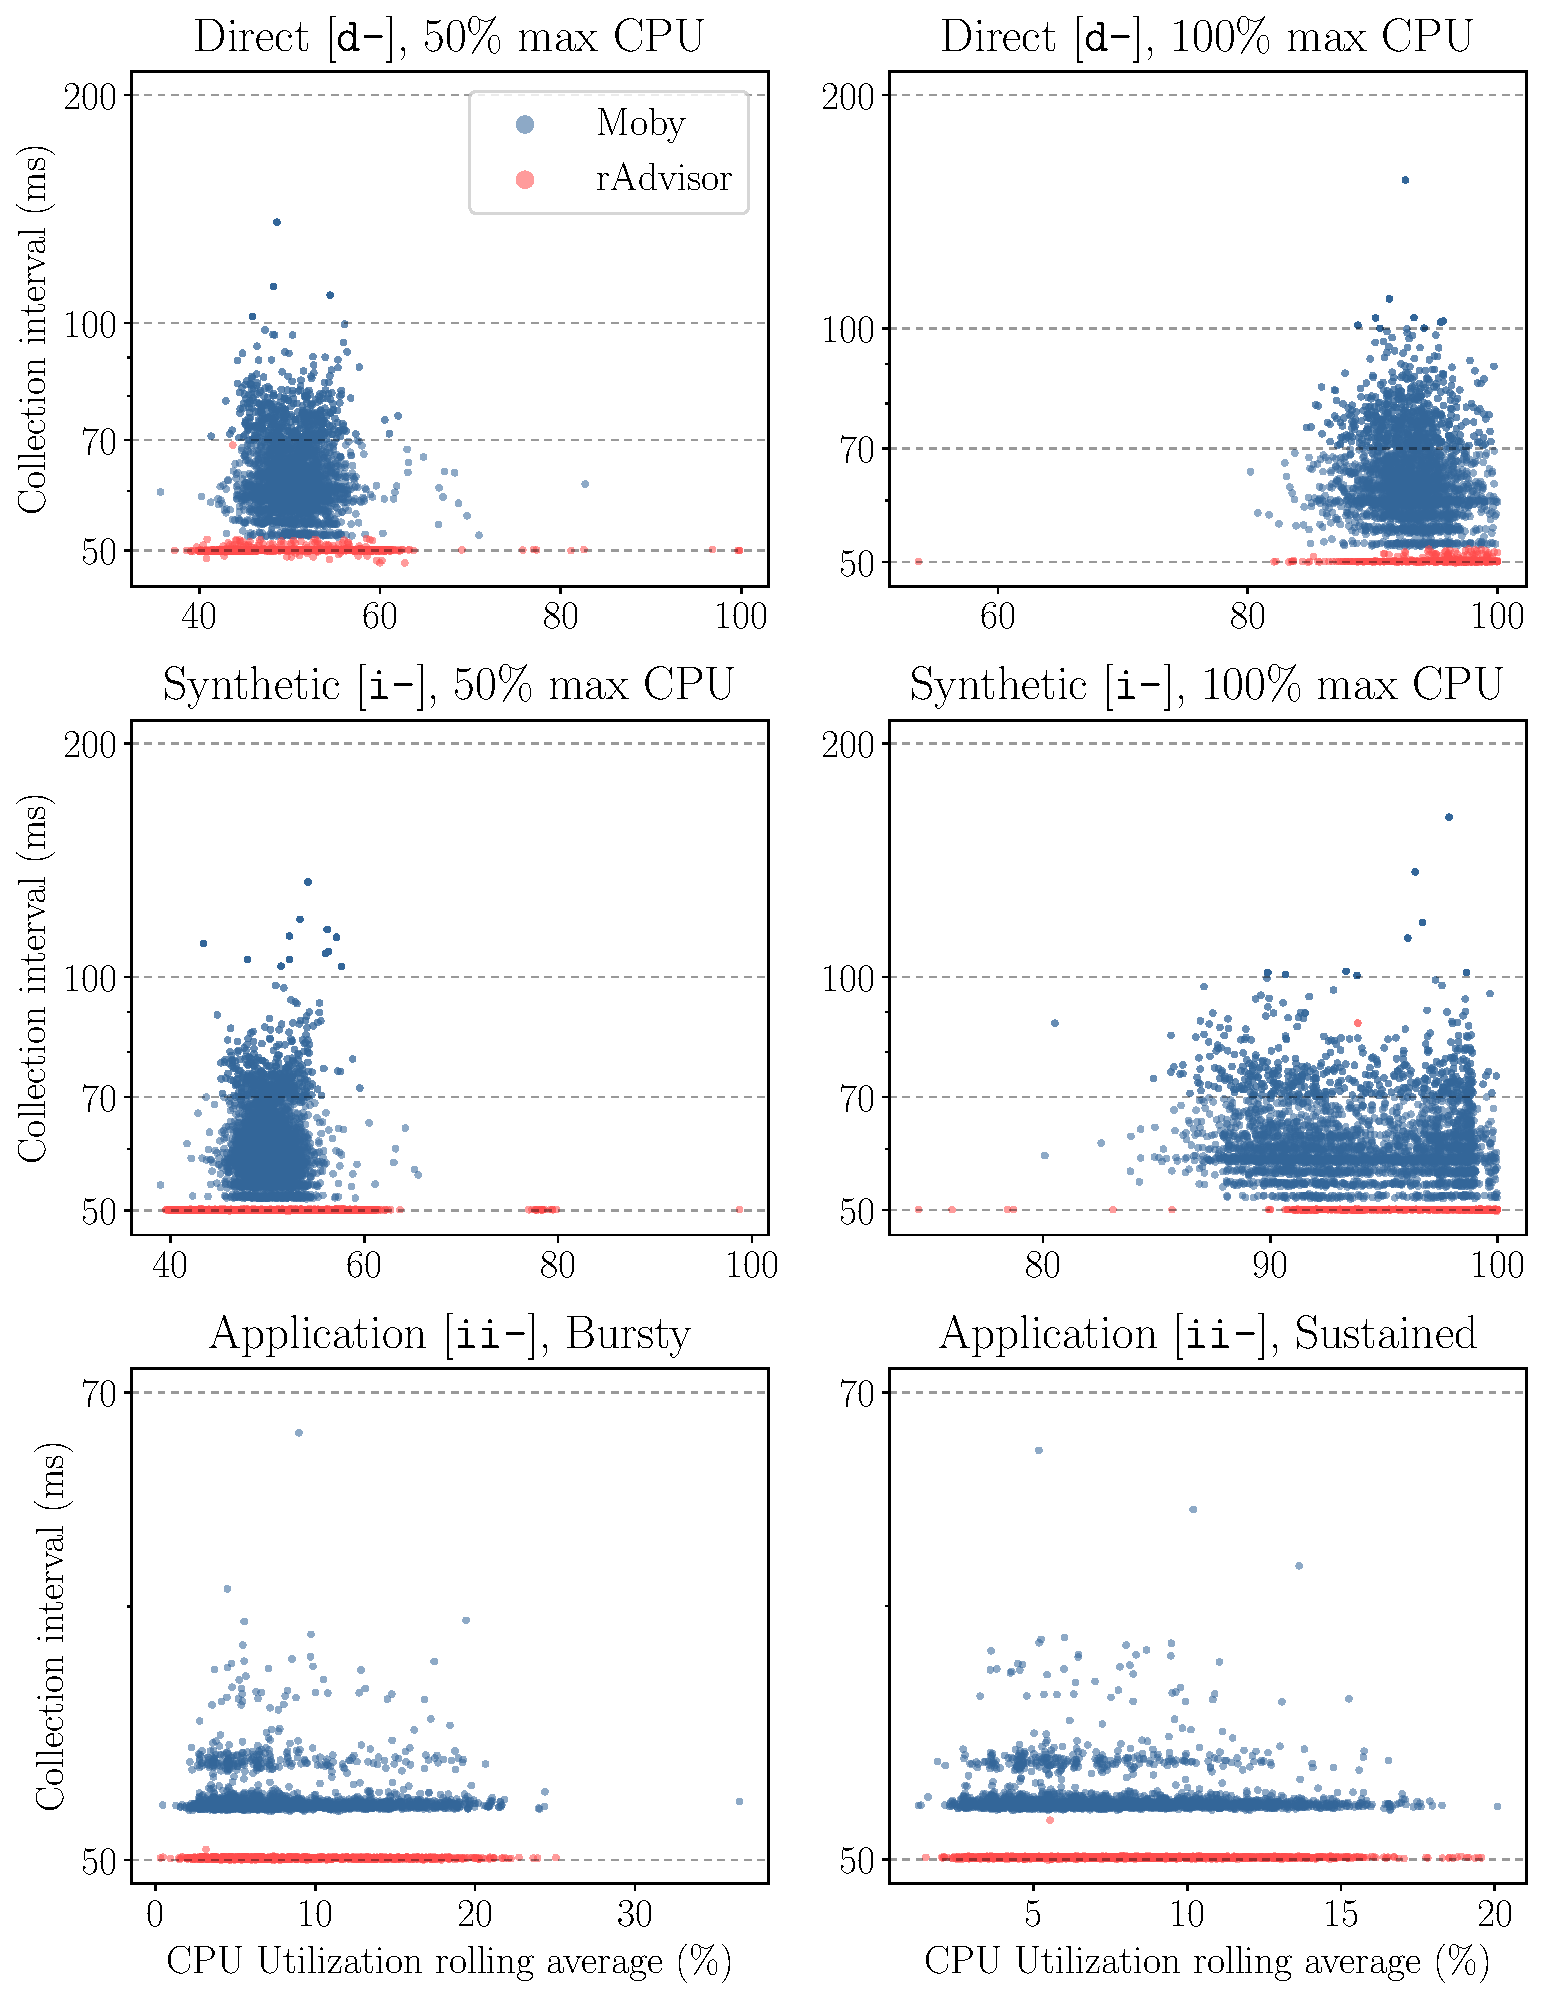
\includegraphics[width=0.97\textwidth]{graphs/cpu_interval_matrix.pdf}
    \vspace{0.7em}
    \caption{
        Set of scatterplots showing the relationship between CPU utilization and observed collection interval
        for both Moby (\textcolor{moby}{blue}) and rAdvisor (\textcolor{radvisor}{red}), with 20\% of all data points shown
    }
    \label{fig:interval_matrix}
    \vspace{1em}
\end{figure}

\begin{aside}
    As an aside, there does appear to be some sort of banding in the scatterplots (especially in the top 4 Moby plots),
    though the cause of this is unknown.
    It's possible there was some number narrowing or rounding error during data analysis,
    though we're not exactly sure what the source is.
    It's also possible that the bands are an artifact of the timing mechanism
    used in the patched Moby version, which utilizes the Golang standard library's concurrency control features.
\end{aside}


\section{Conclusion}

In our project, we've been able to investigate various system resource utilization monitors for Docker containers,
eventually ending up developing our own custom solution in Rust.
In order to be useful for examining the emergence of millibottlenecks in online systems,
our tool needed to operate with \granularity and \overhead,
the primary criteria we used to evaluate the tools.
To examine the tools and compare their ability to meet these criteria,
we performed 360 experiments in CloudLab,
an experiment test bed for cloud research projects.
Each experiment type tested a variety of different configurations
and imposed a handful of both synthetic and application benchmarks.
In the end, our custom-built tool, rAdvisor, provided several advantages over current tools
such as being designed for the specific purpose of monitoring research systems
(unlike current solutions that are built for real-world deployments \cite{SysDig, Cadvisor}).
In direct CPU Utilization, rAdvisor had significantly less direct overhead during periods of load,
and had little to no impact on the distribution of response times in application benchmarks.
Moreover, rAdvisor was significantly more consistent at achieving its target collection interval
than Moby across each test type.
It never degraded past 100 milliseconds (+50 milliseconds from its target)
in the 3 million collection events we observed,
whereas Moby degraded as far as taking seconds between collection events,
causing loss of all collected data during the periods of degradation.
Though it did have an observable impact on the synthetic benchmark of the systems,
we're confident we can reduce that in the future by modifying our underlying implementation (\textit{see Future Work}).

\subsection{Challenges}

Throughout this project we faced many setbacks and challenges that caused us to pivot the scope of our project. 
At the beginning of the semester, our project proposal focused primarily on Kubernetes
and we spent a lot of the first half of the project researching
and implementing a Kubernetes cluster with the WISE microblog benchmark,
yet ended up using none of it in our project.
While researching monitoring tools that provided \granularity and \overhead,
we also spent an excessive amount of time attempting to make cAdvisor, Sysdig, and Moby work to our standards, without avail. 
Having to change our project so far into the semester, 
after observing the lack of tool for monitoring that fit our needs, 
led to us having to complete our implementation very rapidly.
To make this more challenging, we were unfamiliar with the tools and concepts involved,
such as Rust, cgroups, and low-level programming.
A few other challenges we faced were realizing we needed to create some sort of automation to complete our experiments on time
(which we luckily were able to do) and having a large portion of experimental results wiped due to a hard drive failure.

\subsection{Future Work}

If the future, there are a lot of extensions and improvements to be made to the work we completed in this project.
Our original purpose was to integrate Kubernetes with the WISE microblog benchmark to test for millibottlenecks,
although we had to pivot our project halfway. 
Now that we have a tool, rAdvisor, that can monitor with \granularity and \overhead and supports Kubernetes pods,
we can finish developing and running the Kubernetes experiment for the WISE microblog benchmark.
We already made an experimental workflow script for CloudLab that creates an idle Kubernetes cluster on CloudLab,
but with further work, we can investigate the emergence and propagation of millibottlenecks
in containerized (and orchestrated) online systems.

There are also many different improvements that could be made to our experimental workflow.
For one, we could add additional test types to test the relative overhead of rAdvisor and Moby
to investigate if certain application domains are affected differently.
We could look at more target collection intervals (other than 50 milliseconds),
letting us investigate the limits of both tools and see if the target interval affects the overhead and observed granularity.
Alternatively, though we used a microblog benchmark that only had certain parts containerized,
we could fully containerize the application (including the web server frontend and database backend),
letting us test the collection tools on additional application types.
At the end during analysis, we also had some difficulty in normalizing and comparing timestamps between log types---%
in the future, this could be a problem we tackle,
using concurrency control mechanisms to guarantee synchronization between different hosts.

In rAdvisor itself, there are a number of improvements that could be made to improve its performance.
As noted earlier, the synthetic benchmarks showed noticeable performance overhead,
which we believe may be attributed to the design of the polling thread
(which periodically polls the Docker daemon to get a list of active, running containers).
There are a few expensive components to it, such as the bloated Docker API bindings library
and the very expensive asynchronous executor that spawns multiple worker threads to execute HTTP requests.
By replacing these with either a lightweight HTTP client to poll the Docker daemon
or taking the shortcut of just listing the virtual directory for the Docker parent cgroup,
we could eliminate a large portion of the performance overhead of the polling thread.
Additionally, though we attempted to reduce the memory and CPU overhead of the collection thread,
we didn't perform any significant profiling using CPU or memory tools such as Valgrind,
which is a suite of tools for memory debugging, memory leak detection, and profiling \cite{Valgrind}.
By doing this, we could better optimize the runtime overhead of the program as a whole.

Additionally, we could make direct improvements to the versatility of rAdvisor by implementing additional features.
For example, rAdvisor currently lacks the functionality to instrument network statistics for containers,
compared to Moby, which does.
The reasoning for this is because networking isolation in Linux and Docker doesn't use cgroups,
and instead uses entirely different mechanisms (namely, network namespaces)
that would require significant additional complexity \cite{DockerCgroups}.
According to the Docker documentation, instrumentation software would have to fork a new process per container,
switch the network namespace for each, and collect network statistics in those processes.
From here, we would also have to implement IPC and child process control,
which we deemed to be outside of the scope of the current project.
Another possible feature to add would be adapting rAdvisor to also work on Windows systems.
Since 2016, Microsoft has made available a set of high level APIs called Host Compute Services,
used to instantiate and manage first-party Windows containers in the kernel \cite{HCS}
(which is the foundation of Windows functionality for Docker).
With this, Docker containers can be created that run Windows Server,
a niche workflow common in fields such as .NET development.
Using the HCS API, we could add Windows support for system resource utilization instrumentation
to rAdvisor, which already compiles on Windows due to Rust's excellent cross platform support.

\subsection{Final Words}

Throughout the course of this project, we explored the innerworkings of collection tools
such as Sysdig, cAdvisor, Collectl, and Moby.
We soon realized the flaws and saw the need for a tool that could prioritize high granularity and low overhead
while still delivering consistent results.
rAdvisor delivers on all of our goals, and contains many efficiencies necessary for research needs.
Even in the areas that rAdvisor underperforms in,
we have a clear path forward to improve its performance and better optimize it.
We hope that rAdvisor can serve the purpose of a useful collection tool,
and eventually be used to detect millibottlenecks in containerized and orchestrated systems.

\pagebreak
\printbibliography

\pagebreak
\appendix
\section{Artifacts}
\label{app:artifacts}

During the completion of our project, we produced a variety of data, code, and documentation artifacts,
which are listed below:

\subsection{GitHub repositories}
\vspace{0.5em}

\begin{itemize}
    \item \github{elba-docker}{radvisor} -
    repository for rAdvisor, the primary artifact we created for the project,
    which is our custom Rust-based Docker container stats collection tool.
    
    \item \github{elba-docker}{moby} (fork of \github{moby}{moby}) -
    repository for our patched version of Moby, another primary artifact of the project,
    where we introduce configurable automatic statistics collection for running containers.
    
    \item \github{elba-docker}{experiment} (fork of \github{coc-gatech-newelba}{WISETutorial}) -
    contains the experimental workflow Bash scripts, configuration files, and Dockerfiles
    for each of the three test types, which run the experiments in CloudLab cluster.
    Also, the repository contains the (minor) modifications made to the microblog benchmark,
    which are mostly related to the differences in database user inference between
    bare metal and containerized environments
    (since containers run as the \texttt{root} user by default).
    
    \item \github{elba-docker}{automation} -
    contains the Python automation scripts used to automate provisioning and running experiments on CloudLab,
    utilizing Selenium to automate creating and terminating experiments according to a YAML configuration file.
    
    \item \github{elba-docker}{analysis} -
    collection of Python scripts and Jupyter Notebooks used for the parsing and analysis
    of our generated experimental data (used to create the graphs/tables in this report).
    
    \item \github{elba-docker}{instrumentation} -
    working area used over the process of evaluating various system instrumentation for Docker,
    containing benchmarks, log files, and initial parsers/analysis notebooks for Moby, cAdvisor, Sysdig, and rAdvisor.
    
    \item \github{elba-docker}{sysdig} (fork of \github{draios}{sysdig}) -
    contains our minor modification to the upstream Sysdig repository
    where we remove the 100 millisecond lower bound on the collection interval
    
    \item \github{elba-docker}{nbench} (fork of \github{zosxang}{nbench}) -
    contains our pre-compiled Linux-amd64 binary under "Releases" that we use for running nbench in our experiments.
    
    \item \github{elba-docker}{services} (fork of \github{daniel-neelappa}{elbacontainer}) -
    contains the modifications we made to the Dockerfiles for the Elba microblog benchmark application,
    which mostly consist of adding the ability to pass in a database user to the contained microservices.
\end{itemize}

\subsection{Docker containers}

First, there are the five microservice containers built from the modified Dockerfiles
in \github{elba-docker}{services},
which reflect the additional capability to include the database username when running:

\vspace{-0.3em}
\begin{itemize}
    \itemsep-0.1em 
    \item \dockerhub{wisebenchmark}{auth}
    (\href{https://github.com/elba-docker/services/blob/master/auth/dockerfile}{Source Dockerfile})
    \item \dockerhub{wisebenchmark}{inbox}
    (\href{https://github.com/elba-docker/services/blob/master/inbox/dockerfile}{Source Dockerfile})
    \item \dockerhub{wisebenchmark}{queue}
    (\href{https://github.com/elba-docker/services/blob/master/queue/dockerfile}{Source Dockerfile})
    \item \dockerhub{wisebenchmark}{blog}
    (\href{https://github.com/elba-docker/services/blob/master/blog/dockerfile}{Source Dockerfile})
    \item \dockerhub{wisebenchmark}{sub}
    (\href{https://github.com/elba-docker/services/blob/master/sub/dockerfile}{Source Dockerfile})
\end{itemize}

There are also the Docker images used to bootstrap the benchmark containers in \github{elba-docker}{experiment}:

\vspace{-0.3em}
\begin{itemize}
    \item \dockerhub{jazevedo6}{direct\_collectl}
    (\href{https://github.com/elba-docker/experiment/blob/master/experiments/direct_collectl/scripts/Dockerfile}{Source Dockerfile}) -
    used to execute the direct CPU overhead test by pre-installing \texttt{stress} on an Ubuntu base image
    
    \item \dockerhub{jazevedo6}{indirect\_throughput}
    (\href{https://github.com/elba-docker/experiment/blob/master/experiments/indirect_throughput/scripts/Dockerfile}{Source Dockerfile}) -
    used to execute the indirect synthetic benchmark test by pre-installing \texttt{nbench} on an Ubuntu base image
\end{itemize}

\subsection{Data}
\vspace{0.75em}

The final data for the three different experiments types is available on Google Drive at:

\vspace{-0.75em}
\href{https://drive.google.com/open?id=1I8FN0b_y37_vpGmf2XM0oL0W-5GsHbj0}{
\iconGoogleDrive\,drive.google.com/open?id=1I8FN0b\_y37\_vpGmf2XM0oL0W-5GsHbj0}

\subsection{Compiled binaries}
\vspace{0.5em}

\begin{itemize}
    \item \href{https://github.com/elba-docker/experiment/tree/master/artifacts}{Patched moby Debian (\texttt{.deb}) packages} -
    we used the existing tools at \github{docker}{docker-ce}
    to build Debian packages for our custom version of Moby,
    which we then install during experiment execution on the Ubuntu bare metal hosts.
    
    \item \href{https://github.com/elba-docker/radvisor/releases}{rAdvisor binaries} -
    we use GitHub actions to automatically build and distribute binaries of rAdvisor upon release,
    which we then directly download and run during experiment execution.
\end{itemize}

\subsection{Supplemental documentation}

During development, we wrote detailed documentation on each column in the rAdvisor output logs,
documenting which cgroup file they come from and what they mean.
The documentation is available here: 
\href{https://github.com/elba-docker/radvisor/blob/develop/docs/collecting.md}{\faGithub~elba-docker/radvisor/docs/collecting.md}

We also wrote documentation on the command-line usage of rAdvisor, which is available here:
\href{https://github.com/elba-docker/radvisor/tree/develop/man}{\faGithub~elba-docker/radvisor/man/}

\end{document}
